%----------------------------------------------------------------------------------------
%	PACKAGES AND OTHER DOCUMENT CONFIGURATIONS
%----------------------------------------------------------------------------------------

\documentclass[paper=a4, fontsize=11pt]{scrartcl} % A4 paper and 11pt font size

\usepackage[margin=1.0in]{geometry}	%for some reason, looks beter. 

\usepackage[T1]{fontenc} % Use 8-bit encoding that has 256 glyphs
\usepackage{fourier} % Use the Adobe Utopia font for the document - comment this line to return to the LaTeX default
\usepackage[english]{babel} % English language/hyphenation
\usepackage{amsmath,amsfonts,amsthm} % Math packages

\usepackage{lipsum} % Used for inserting dummy 'Lorem ipsum' text into the template

\usepackage{sectsty} % Allows customizing section commands
\allsectionsfont{\centering \normalfont\scshape} % Make all sections centered, the default font and small caps

\usepackage{fancyhdr} % Custom headers and footers
\pagestyle{fancyplain} % Makes all pages in the document conform to the custom headers and footers
\fancyhead{} % No page header - if you want one, create it in the same way as the footers below
\fancyfoot[L]{} % Empty left footer
\fancyfoot[C]{} % Empty center footer
\fancyfoot[R]{\thepage} % Page numbering for right footer
\renewcommand{\headrulewidth}{0pt} % Remove header underlines
\renewcommand{\footrulewidth}{0pt} % Remove footer underlines
\setlength{\headheight}{13.6pt} % Customize the height of the header

\numberwithin{equation}{section} % Number equations within sections (i.e. 1.1, 1.2, 2.1, 2.2 instead of 1, 2, 3, 4)
\numberwithin{figure}{section} % Number figures within sections (i.e. 1.1, 1.2, 2.1, 2.2 instead of 1, 2, 3, 4)
\numberwithin{table}{section} % Number tables within sections (i.e. 1.1, 1.2, 2.1, 2.2 instead of 1, 2, 3, 4)

\setlength\parindent{0pt} % Removes all indentation from paragraphs - comment this line for an assignment with lots of text

%----------------------------------------------------------------------------------------
%Personal Packages and File Dependencies 
%----------------------------------------------------------------------------------------	

\usepackage{graphicx}	%insert graphics
%\usepackage{microtype}	%improves spacing
\usepackage{float}		%H postion	
\usepackage{caption}	%caption w/o : 	
\usepackage{framed}		%creates frames
\usepackage{enumitem}

\usepackage{listings}	%insert sourcecode
\usepackage{color}
\usepackage{pdfpages}	%include PDF pages

\usepackage{bigstrut}	%exce2latex table packages
\usepackage{rotating}
\usepackage{multirow}
\usepackage{booktabs}
\usepackage[framed]{mcode}

\usepackage{cleveref}	%cooler references, needs to be last
\usepackage[bookmarks]{hyperref}
\graphicspath{{../Figures/}{../figures/}} % This automatically connects to the figure folder

%----------------------------------------------------------------------------------------
%	TITLE SECTION
%----------------------------------------------------------------------------------------

\newcommand{\horrule}[1]{\rule{\linewidth}{#1}} % Create horizontal rule command with 1 argument of height

\title{	
\normalfont \normalsize 
\textsc{TEMPLE UNIVERSITY COLLEGE OF ENGINEERING | ECE 3522 | SPRING 2015} \\ [25pt] % Your university, school and/or department name(s)
\horrule{0.5pt} \\[0.4cm] % Thin top horizontal rule
\huge Computer Assignment 2: Regression and Histograms \\ % The assignment title
\horrule{2pt} \\[0.5cm] % Thick bottom horizontal rule
}

\author{Tyler Berezowsky} % Your name

\date{\normalsize\today} % Today's date or a custom date

\begin{document}
\maketitle % Print the title

\section{Problem Statement} 
%Summarize the problem statement in one paragraph. Clearly state what the knowns are and what unknowns you must find.
This computer assignment consisted of two tasks focused around ``basic prediction functions''. The first task was to overlay the global mean and a linear regression on the closing Google stock prices acquired through the frame and windowing exercise of CA: 01. The second task was to develop a probability mass function (pmf) or histogram, and the cumulative  distribution function for the audio signal also from the previous computer assignment. 


\section{Approach and Results} 
%Describe your approach to finding the unknowns. Use numbered figures, tables and equations where necessary.

\text{\normalfont\scshape Google Stock Prices:} \\
As stated in the problem statement, the stock prices were previously filtered via the frame and window technique. The frame and window metrics were 1 and 7 respectively. The global mean was calculated through the \verb|mean()| command. The linear regression was calculated  via the command \verb|fitlm|. The resulting computations can be seen in figure~\ref{fig: liner_regression}. 

\begin{figure}[h] % linear regression
	\centering 
	\includegraphics[width=\linewidth]{lg_01}
	\caption{Plot of Google stock price frame and windowed, overlaid with the global mean and a linear regression.}
	\label{fig: liner_regression} 
\end{figure}

The plot depicts the original signal (blue),  the mean (orange): a single term approximation, and the linear regression (yellow): a two term approximation. The mean is constant for all time, while the linear regression attempts to crudely track the signal with time. \\

\text{\normalfont\scshape Audio Signal:} \\
Generation of the histogram / probability mass function and cumulative mass function was also preformed all with a built-in MATLAB commands, \verb|histogram|. Two histogram plots were generated. The first with a bin size of 500, and the second with the requested bin size of 10. Plots of the histograms along with their corresponding cumulative distribution function can be seen in figures~\ref{fig: hist_500} and \ref{fig: histo_10}. 

\begin{figure}[H] % binwidth = 500 
	\centering 
	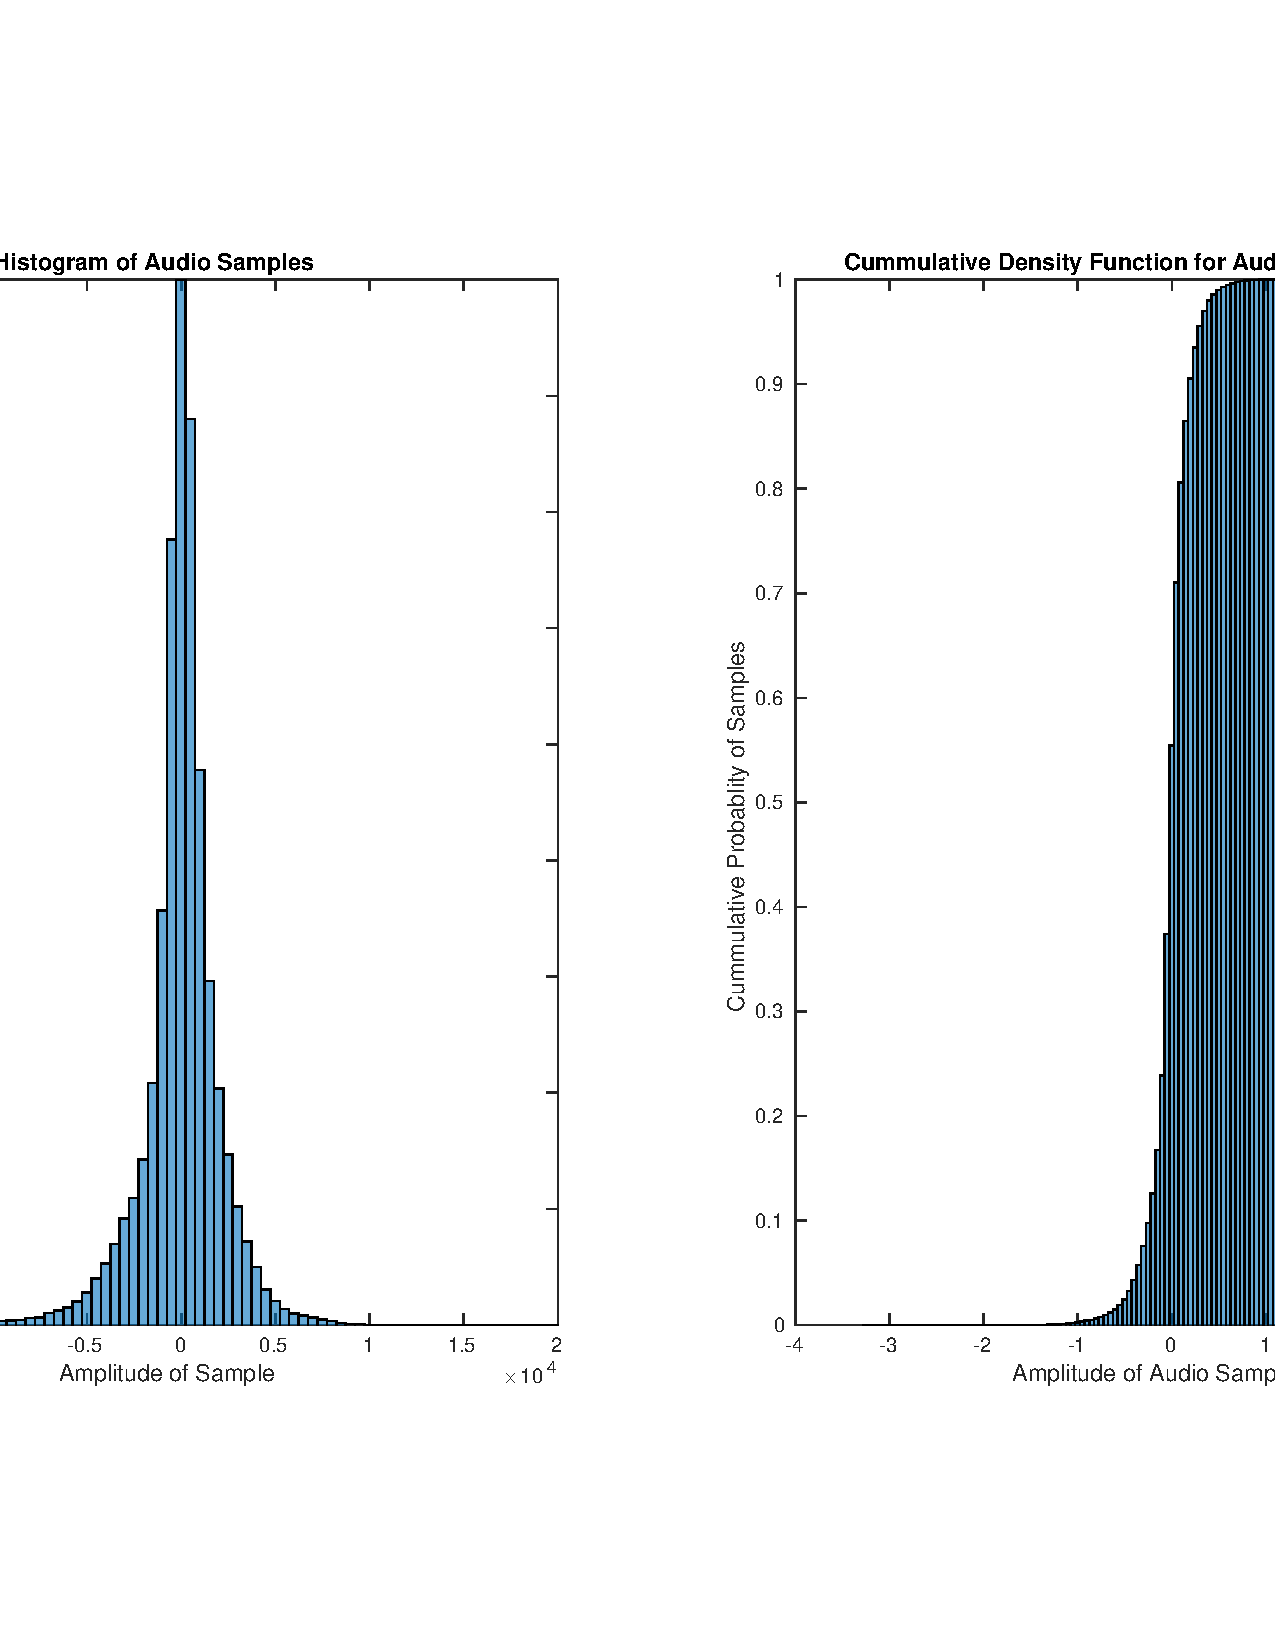
\includegraphics[width=\linewidth]{histo_01.png}
	\caption{Histogram plot emulating the probability mass distribution with a bin width of 500 (left). Cumulative distribution function for the pmd (right).}
	\label{fig: hist_500} 
\end{figure}

\begin{figure}[H] % binwidth = 10 
	\centering 
	\includegraphics[width=\linewidth]{histo_02.png}
	\caption{Histogram plot emulating the probability mass distribution with a bin width of 10 (left). Cumulative density function for the pmd (right). }
	\label{fig: histo_10} 
\end{figure}

The following relationships can be noted from the figures. The bin width of a histogram plot is proportional to the probability of bin. This can be seen through the scaling of the two figures. The bin width also determines the readability of the chart for large data sets. If the bin width is too small, as in figure~\ref{fig: histo_10}, it becomes unreadable. The histograms are not symmetrical with a tendency for negative amplitudes. The distribution resembles a bell curve, but as it lacks symmetry and the decreasing rate of increase near the mean or max extrema, it cannot be classified as Gaussian. In physical correlation, the amplitude values closest to zero, have the highest probabilities. This is supported by the zero crossing nature of AC signals and the near-zero mean found in CA: 01.  

\section{MATLAB Code} 
%Show and briefly explain your MATLAB code.
As evident in the results section, the tasks were completed with built-in MATLAB commands primarily from the statistics toolbox or with code from the previous computer assignment. The only interesting development was the use of the \verb|histogram()| command which generates a histogram or cumulative distribution function based on the arguments given. 

\lstinputlisting[caption=Code for CA\_02.m]{../MATLAB/ca_02.m}

\section{Conclusions} 
%Summarize what you found.
The mean as a rudimentary signal approximation is not very effective. Consisting of only a constant, it does not vary with time, and therefore lacks a non-zero first derivative delivering no rate information. The linear approximation includes time as a factor, $y = mx + b$, but delivers only the most primitive approximation ignoring any local extrema in a signal, and local extrema in stock prices is the gold of the craft.  In addition, if the signal's mean was zero, as in the audio signal, a linear approximation would provide no predictive information. This type of analysis is only for signals with relatively constant trends. \\


The carnality of a data set will determine the extent of resolution required for a histogram plots useability. The number of bins in a histogram chart is determined by the following factors: the number of possibilities in the data set and the number of possibilities each bin is set to represent or the bin width. If the cardinality of the data set is large as with an audio signal and the bin size is small, the width of each bin will become indistinguishable. Increasing the bin width will decrease the resolution for each bin, but allows the bins to become discernible. This effect is displayed in figures~\ref{fig: hist_500} and \ref{fig: histo_10}. Also illustrated by the two example plots is the inverse relationship between the number of bins and the probability of a specific bin. As the number of bins for a histogram chart increases, the number of possibilities each bin represents decreases thus the probability for that bin decreases. 

\end{document}